
\chapter{Polytope resolution strategies} % Main chapter title

\label{ch:polytope_algorithms} % Change X to a consecutive number; for referencing this chapter elsewhere, use \ref{ChapterX}

\section{Polytope evaluation}

\begin{figure}[!htb]
    \centering
    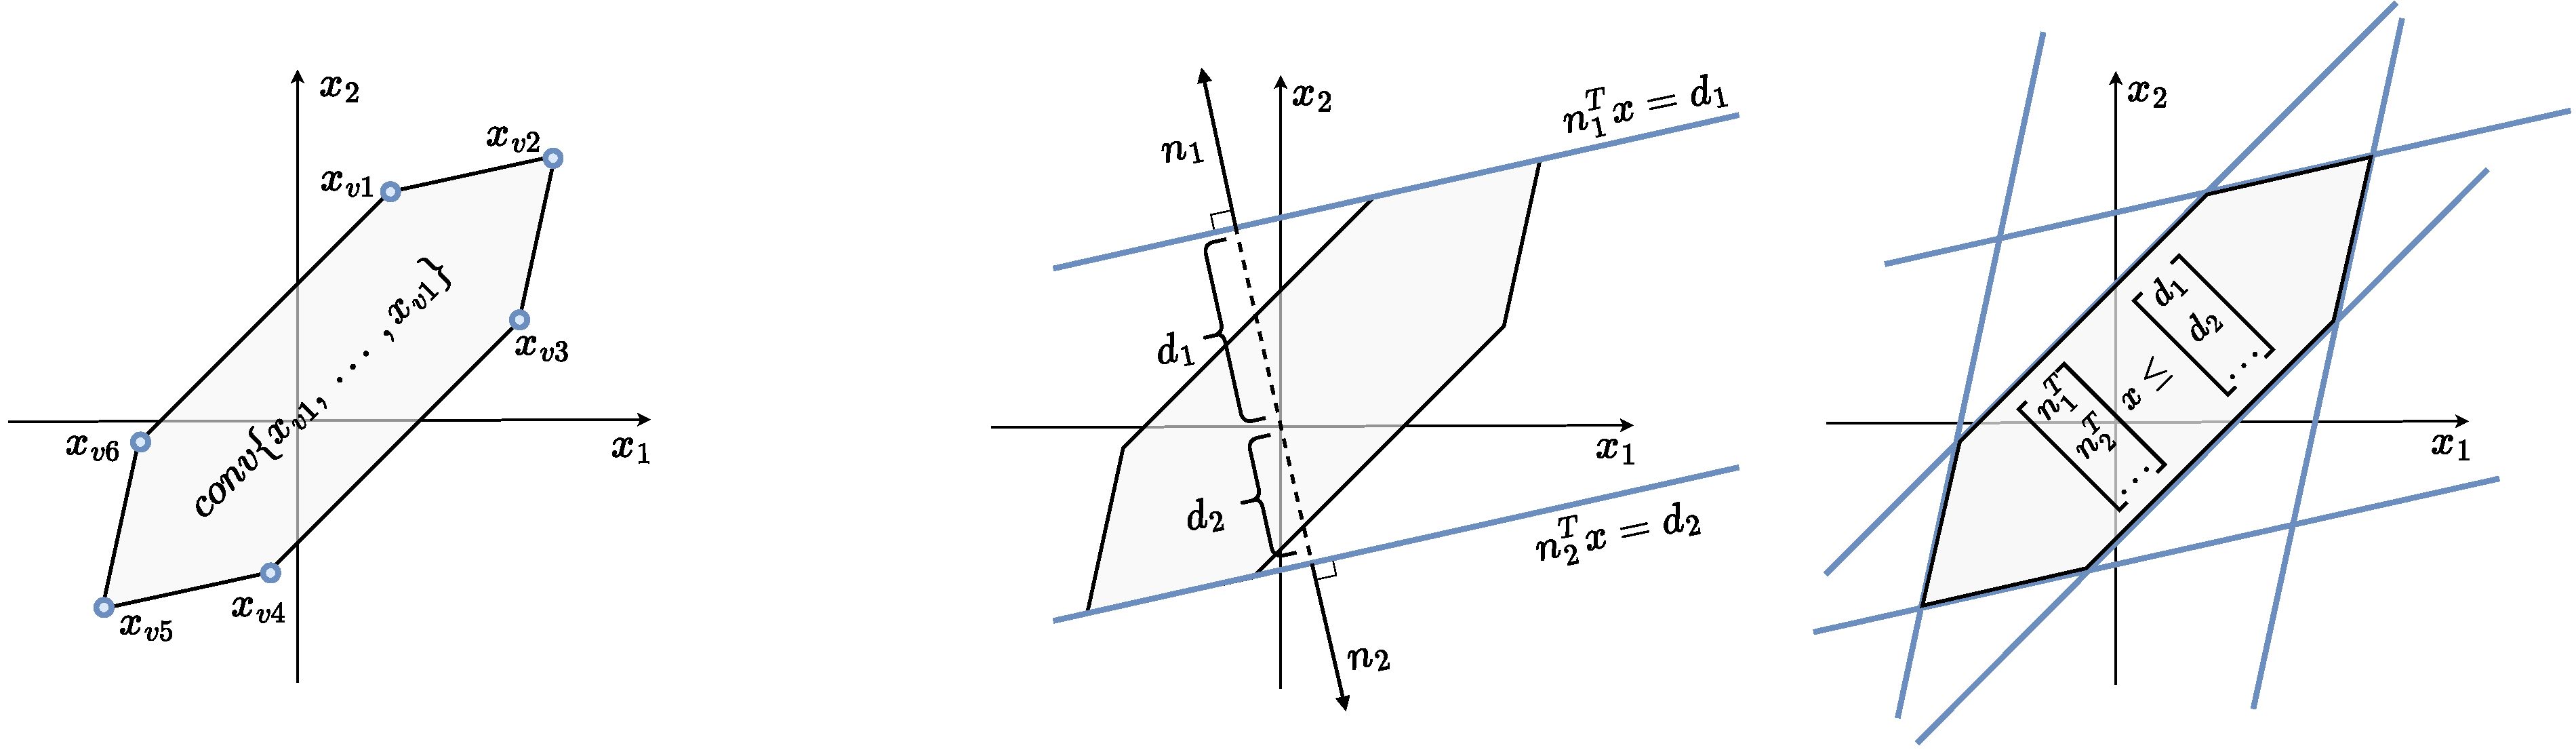
\includegraphics[width=\linewidth]{Chapters/imgs/h_v_rep.pdf}
    \caption{Caption}
    \label{fig:hv_rep}
\end{figure}

Two most common ways of representing a convex polytope $\mathcal{P}_x$ are $\mathcal{V}$-representation and $\mathcal{H}$-representation. $\mathcal{V}$ or vertex representation consist in specifying a list of polytope's vertices, where the polytope $\mathcal{P}_x$ is defined as their convex hull 
\begin{equation}
    \mathcal{P}_x = conv\{ \bm{x}_{v1},~\bm{x}_{v2},~ \ldots , ~\bm{x}_{vN} \}
\end{equation} 

$\mathcal{H}$ or half-plane representation, on the other hand, is defined as the intersection of the half-planes forming the faces of the polytope
\begin{equation}
    \mathcal{P}_x = \{ H\bm{x} \leq \bm{d} \}
\end{equation} 
Where the matrix $H$ is composed of the normal vectors $\bm{n}_i^T$ of the half-planes and the vector $\bm{d}$ contains their displacement $d_i$ from the origin. The $\mathcal{V}$ and $\mathcal{H}$ representation of an example 2-dimensional polytope is shown Figure \ref{fig:hv_rep}. 

Polytope $\mathcal{V}$-representation, in the case of physical ability metrics, are mostly used for visualisation purposes. The vertices can be easily transformed into triangulated meshes and visualised in standard visualisation tools alongside the robot or human models which performance is being evaluated.  $\mathcal{H}$-representation, on the other hand, is more useful for control and optimisation applications. As the polytope is represented by the set of convex linear constraints it can be easily integrated in different optimisation problems. The polytope resolution therefore consists in finding the appropriate polytope representation for a given application. 

In case of physical ability metrics, most polytopes are described as a set of inequality and equality constraints, which in order to be used need to be transformed to an appropriate representation $\mathcal{V}$ or $\mathcal{H}$. However, the choice of the polytope transformation algorithm will therefore highly depend on the polytope formulation (projection or intersection), the nature of the input space limits $\mathcal{I}$ (hypercube or polytope), the polytope representation needed ($\mathcal{V}$ or $\mathcal{H}$) as well as the required computational efficiency.


\section{Strategies for polytope evaluation}
\subsection{Intersection formulation $Ax=y$ with hypercube limits $\mathcal{I}$}

\begin{figure}[!htb]
    \centering
    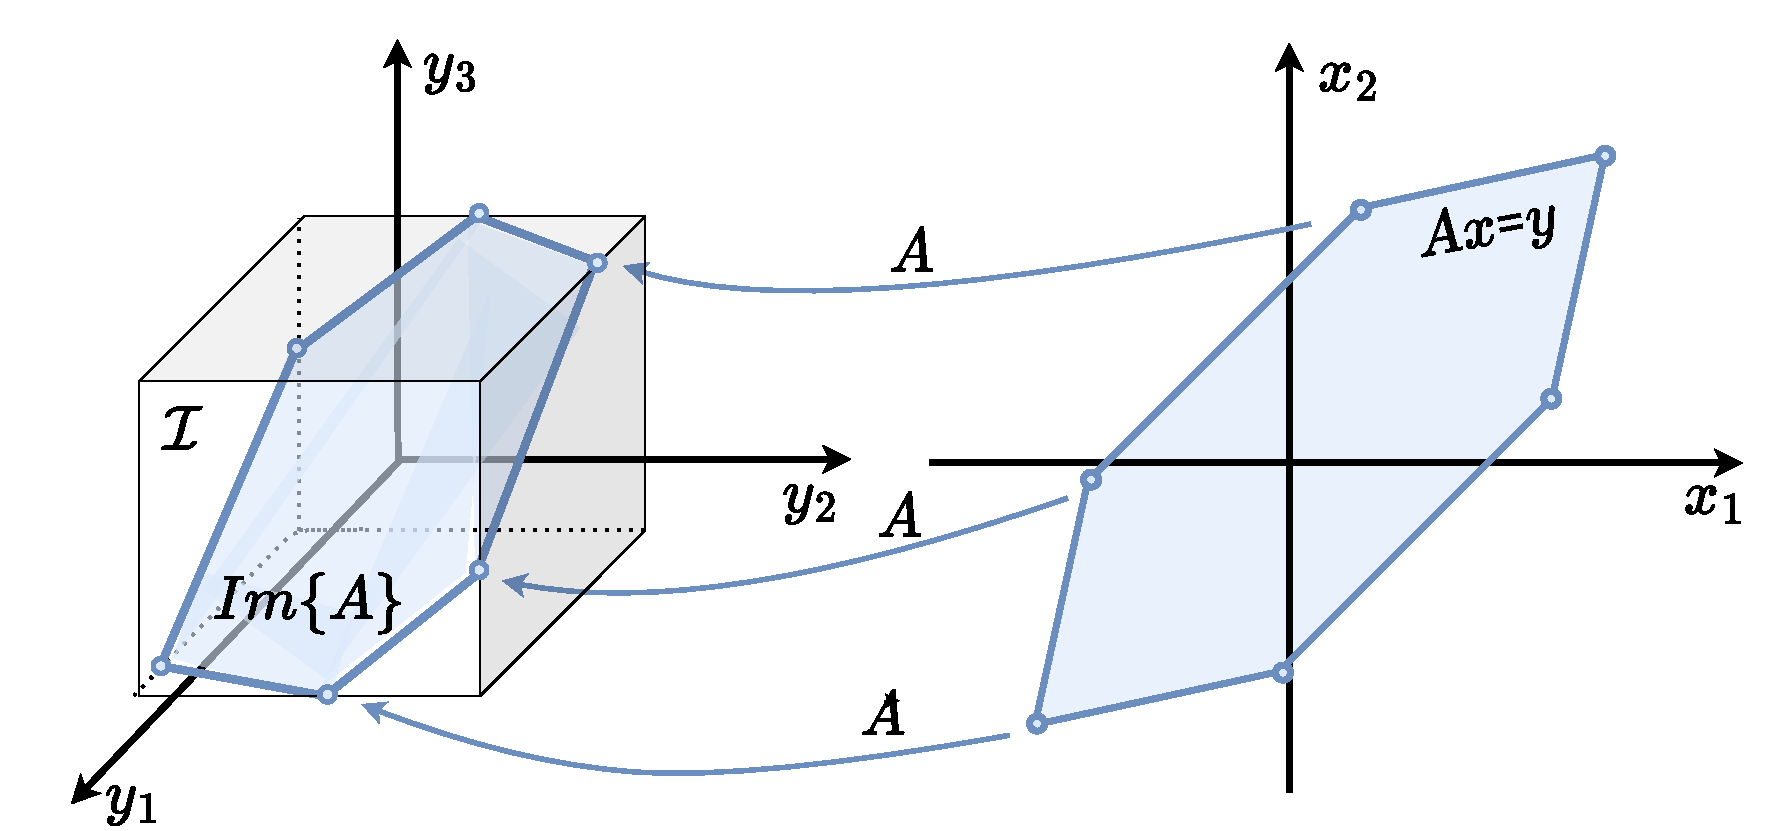
\includegraphics[width=0.8\linewidth]{Chapters/imgs/intersection.pdf}
    \caption{Caption}
    \label{fig:inter}
\end{figure}

The intersection polytope formulation (\ref{eq:inter_poly}) with the hypercube limits (\ref{eq:hypercube_lim}) is a spacial case of the intersection polytope where the input space limits $\mathcal{I}$ are defined as independent min-max ranges 

\begin{equation}
    \mathcal{P}_x=\{\bm{x} |~ A\bm{x} = \bm{y},~\bm{y}_{min} \leq  \bm{y} \leq \bm{y}_{max}  \}
    \label{eq:inter_hyp}
\end{equation}


The geometrical representation of the polytope $\mathcal{P}_x$ defined by (\ref{eq:inter_hyp}) is shown on Figure \ref{fig:inter}, for an example $n=3$ dimensional hypercube $\mathcal{I}$ and $m=2$ dimensional polytope $\mathcal{P}_x$. 
The resulting polytope $\mathcal{P}_x$ is an affine projection of the intersection of the hypercube $\mathcal{I}$ and the image of the matrix $A$ ($Im\{A\}$) into the lower dimensional output space. As shown on Figure \ref{fig:inter}, the vertices and faces of the polytope $\mathcal{P}_x$ do not correspond to the projection of the vertices and faces of the hypercube $\mathcal{I}$. Rather, as show in in equation (\ref{eq:proj_inter}), there is a unique mapping between the vertices and faces of the intersection of the hypercube $\mathcal{I}$ and the image of the matrix $A$ and the vertices and the faces of the polytope $\mathcal{P}_x$, given through the Moore-Penrose inverse of the matrix $A$. 

\paragraph*{$\mathcal{H}$-representation} Finding the $\mathcal{H}$-representation of such polytope can be done directly by substituting $\bm{y}$ with $A\bm{x}$ in the hypercube equation (\ref{eq:hypercube_lim}) and rewriting it in the matrix from
\begin{equation}
   \underbrace{\begin{bmatrix}
        A\\
        -A
    \end{bmatrix}}_{H}\bm{x} \leq \underbrace{\begin{bmatrix}
         \bm{y}_{max}\\
        -\bm{y}_{min} 
    \end{bmatrix} }_{\bm{d}}
\end{equation}
resulting in the polytope defined with its $\mathcal{H}$-representation
\begin{equation}
    \mathcal{P}_x=\{\bm{x} |~ H\bm{x} \leq \bm{d} \}
    \label{eq:inter_h_rep}
\end{equation}
Even though this $\mathcal{H}$-representation (\ref{eq:inter_h_rep}) of the polytope $\mathcal{P}_x$ follows directly from its definition and can be easily expressed, it might not be minimal. This means that even though the equation (\ref{eq:inter_h_rep}) is correct and fully describes the polytope $\mathcal{P}_x$, there might be some redundant half-plane constraints $n_i^T\bm{x}\leq d_i$. Many algorithms have been developed over the years for removing the redundant constraints $H\bm{x}\leq\bm{d}$ \cite{Paulraj2006}, and their computational complexity is generally equivalent to solving a series of linear programming (LP) problems \cite{Telgen1983}. Therefore, depending on the application and the computational complexity of the polytope description necessary, such techniques can be used to reduce the equation (\ref{eq:inter_h_rep}) to the minimal set of linear constraints $H\bm{x}\leq \bm{d}$.
 
\paragraph*{$\mathcal{V}$-representation} 
One of the most commonly used method for vertex enumeration of this polytope formulation is the double description method \cite{avis_pivoting_nodate} introduced by Fukuda and Avis. It formulates the vertex search problem as transformation of a half-plane representation to a vertex representation, leveraging the fact that the half-plane representation (\ref{eq:inter_h_rep}) can be easily obtained. This generic formulation is well suited and relatively efficient for different high and low dimensional problems. However, when it comes to computational efficiency, methods that show the best results are often the ones leveraging the specific geometry of their problems. 

An efficient algorithm for vertex enumeration of the intersection type polytope has been proposed by Gouttefarde et al. \cite{gouttefarde_versatile_2015} for the use case in the redundancy resolution of the cable driven parallel robots, where the the matrix $A$ is the cable null-space projector of the wrench matrix $N=null\{W\}$, input vector $\bm{y}$ is the vector of cable tensions $\bm{t}$ and the output vector $\bm{x}$ corresponds to the null-space vector $\bm{\lambda}$. This algorithm exploits the geometry of the problem assuming that the wrench matrix null-space is always 2 dimensional, in which case the polytope becomes a 2D polygon, which boundaries are then efficiently navigated in search for extremities. However, this algorithm does not scale well to higher dimensional problems.

In the case of the robotic manipulator's wrench polytope, which has the intersection formulation, as well, where the matrix $A$ is the jacobian transpose matrix $J^T$, the input vector $\bm{y}$ is the vector of joint torques $\bm{\tau}$ and the output vector $\bm{x}$ is a vector of cartesian wrenches $\bm{f}$. For this problem, Chiacchio et al. \cite{chiacchio_evaluation_1996} have proposed an algorithm for finding its vertices that performs an exhaustive search through the input hypercube limits $\mathcal{I}$. This algorithm has been improved by Sasaki et al. \cite{sasaki_vertex_nodate} where the computational complexity has been significantly reduced by exploiting the geometry of the intersection of the hypercube $\mathcal{I}$ and the image of matrix $Im\{A\}$, leveraging the polytope formulation (\ref{eq:proj_inter})
\begin{equation}
\mathcal{P}_x=\{\bm{x} |~ \bm{x} = A^+\bm{y},~ \bm{y} \in Im\{A\}\cap[\bm{y}_{min},\bm{y}_{max}]\}
\label{eq:inter_hyp_inter}
\end{equation}
\todo[inline]{
Building on top of this algorithm, Skuric et al. \cite{skuric2021} have further improved its performance by performing the search in the $n-m$ dimensional \textit{null-space} of the matrix $A$, making this algorithm capable of finding the manipulator's wrench polytope vertices in real-time.}

In the absence of the exact method for finding the polytope's $\mathcal{H}$ or $\mathcal{V}$-representation with an acceptable execution time for the given application, polytope approximation strategies described in Chapter \ref{ch:approximation_algos} may present a viable solution. 

\subsection{Projection formulation $x=By$ with hypercube limits $\mathcal{I}$}
\begin{figure}[!htb]
    \centering
    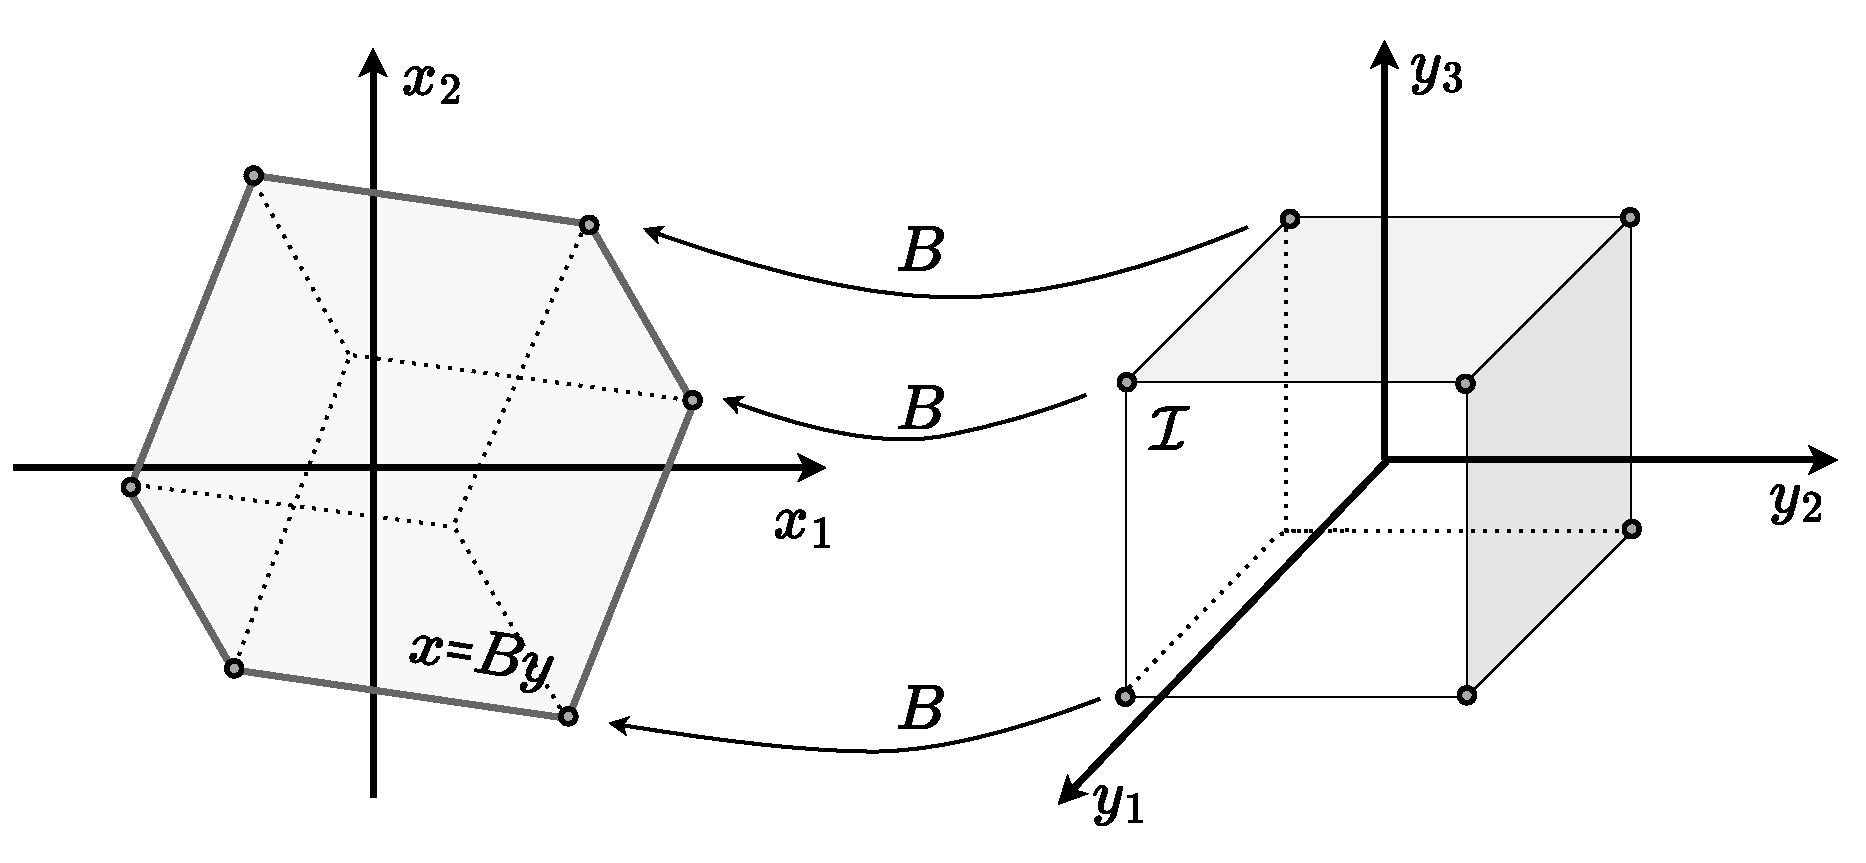
\includegraphics[width=0.8\linewidth]{Chapters/imgs/projection.pdf}
    \caption{Caption}
    \label{fig:proj}
\end{figure}

The projection polytope formulation (\ref{eq:proj_poly}) with the hypercube limits (\ref{eq:hypercube_lim}) is a spacial case of the projection polytope where the input space limits $\mathcal{I}$ are defined as independent min-max ranges 

\begin{equation}
    \mathcal{P}_x=\{\bm{x} |~ \bm{x} = B\bm{y},~\bm{y}_{min} \leq  \bm{y} \leq \bm{y}_{max}  \}
    \label{eq:proj_hyp}
\end{equation}

The geometrical representation of the polytope $\mathcal{P}_x$ defined by (\ref{eq:proj_hyp}) is shown on Figure \ref{fig:proj}, for an example $n=3$ dimensional hypercube $\mathcal{I}$ and $m=2$ dimensional polytope $\mathcal{P}_x$. The resulting polytope $\mathcal{P}_x$ is an affine projection of the hypercube $\mathcal{I}$ into the lower dimensional output space. And all the vertices and the faces of the polytope $\mathcal{P}_x$ correspond directly to the projection of the vertices and faces of the hypercube $\mathcal{I}$. 
 
\paragraph*{$\mathcal{V}$-representation} Finding the vertices of the projection polytope $\mathcal{P}_x$ can be done enumerating the $2^n$ vertices of the hypercube $\mathcal{I}$, by creating a list of all the combinations of the minimal and maximal values of $\bm{y}$, projecting them to the lower dimensional output space $x \in R^m$ using the projection matrix $B$, and calculating the convex-hull of the projected points. The complexity of this approach depend on two factors. The dimension of the of the input space $\bm{y} \in R^n$ and the dimension of the output space $\bm{x}\in R^m$. The number of vertices of the hypercube is grows exponentially $2^n$ with the dimension of the input space $n$, and constructing a matrix of $2^n \times n$ entries can become impractical. On the other hand, as this approach requires a convex-hull algorithm to be run in the $m$-dimensional output space, the dimension $m$ might make the convex-hull algorithm impractical as their complexity grows significantly with the dimension of the space $m$ \cite{Barber1996}.

Therefore for higher dimensional input and output spaces it might be more efficient to first calculate the $\mathcal{H}$-representation  of this polytope, using the methods described in the following section, and then use a vertex enumeration method such as Double-Description Method (DDM) \cite{fukuda_dd} to find the $\mathcal{V}$-representation.

\paragraph*{$\mathcal{H}$-representation} A naive approach to finding the $\mathcal{H}$-representation of the projection formulation (\ref{eq:proj_hyp}) is to decouple the problem and first find the vertex representation of the polytope $\mathcal{P}_x$ and then use the standard vertex enumeration algorithms such as DDM \cite{fukuda_dd} to find the $\mathcal{H}$-representation.

However, more efficient solutions for finding the half-plane representation of the projection formulation (\ref{eq:proj_hyp}) directly are well studied problem in literature. One of the most well known algorithms for this specific case is arguably Fourier-Motzkin elimination (FME), described by Dantzig and Eaves \cite{dantzig1973fourier}. This algorithm uses an iterative inequality elimination method to isolate the set of half-plane equations bounding the polytope $\mathcal{P}_x$. However, this approach has a significant complexity and does not guarantee minimal representation \cite{Monniaux2010}. 
A more efficient algorithm was introduced Bouchard et al. \cite{Bouchard2009} and improved by Gouttefarde and Krut \cite{hyper_psm}, called Hyper-Plane Shifting Method (HPSM). This algorithm finds the minimal $\mathcal{H}$-representation of the polytope (\ref{eq:proj_hyp}) by efficiently performing the exhaustive search of all the possible half-plane combinations. Even-though much more efficient than the Fourier-Motzkin elimination, as it relies on the exhaustive search, it has exponential complexity with the dimension $n$ of the input hypercube $\mathcal{I}$.

Like in the case of the intersection formulation, when the exact methods do not satisfy the time efficiency of a given application, polytope approximation strategies described in Chapter \ref{ch:approximation_algos} may present a viable solution. 

\subsection{Intersection formulation $Ax=y$ with polytope limits $\mathcal{I}$}

\begin{figure}[h]
    \centering
    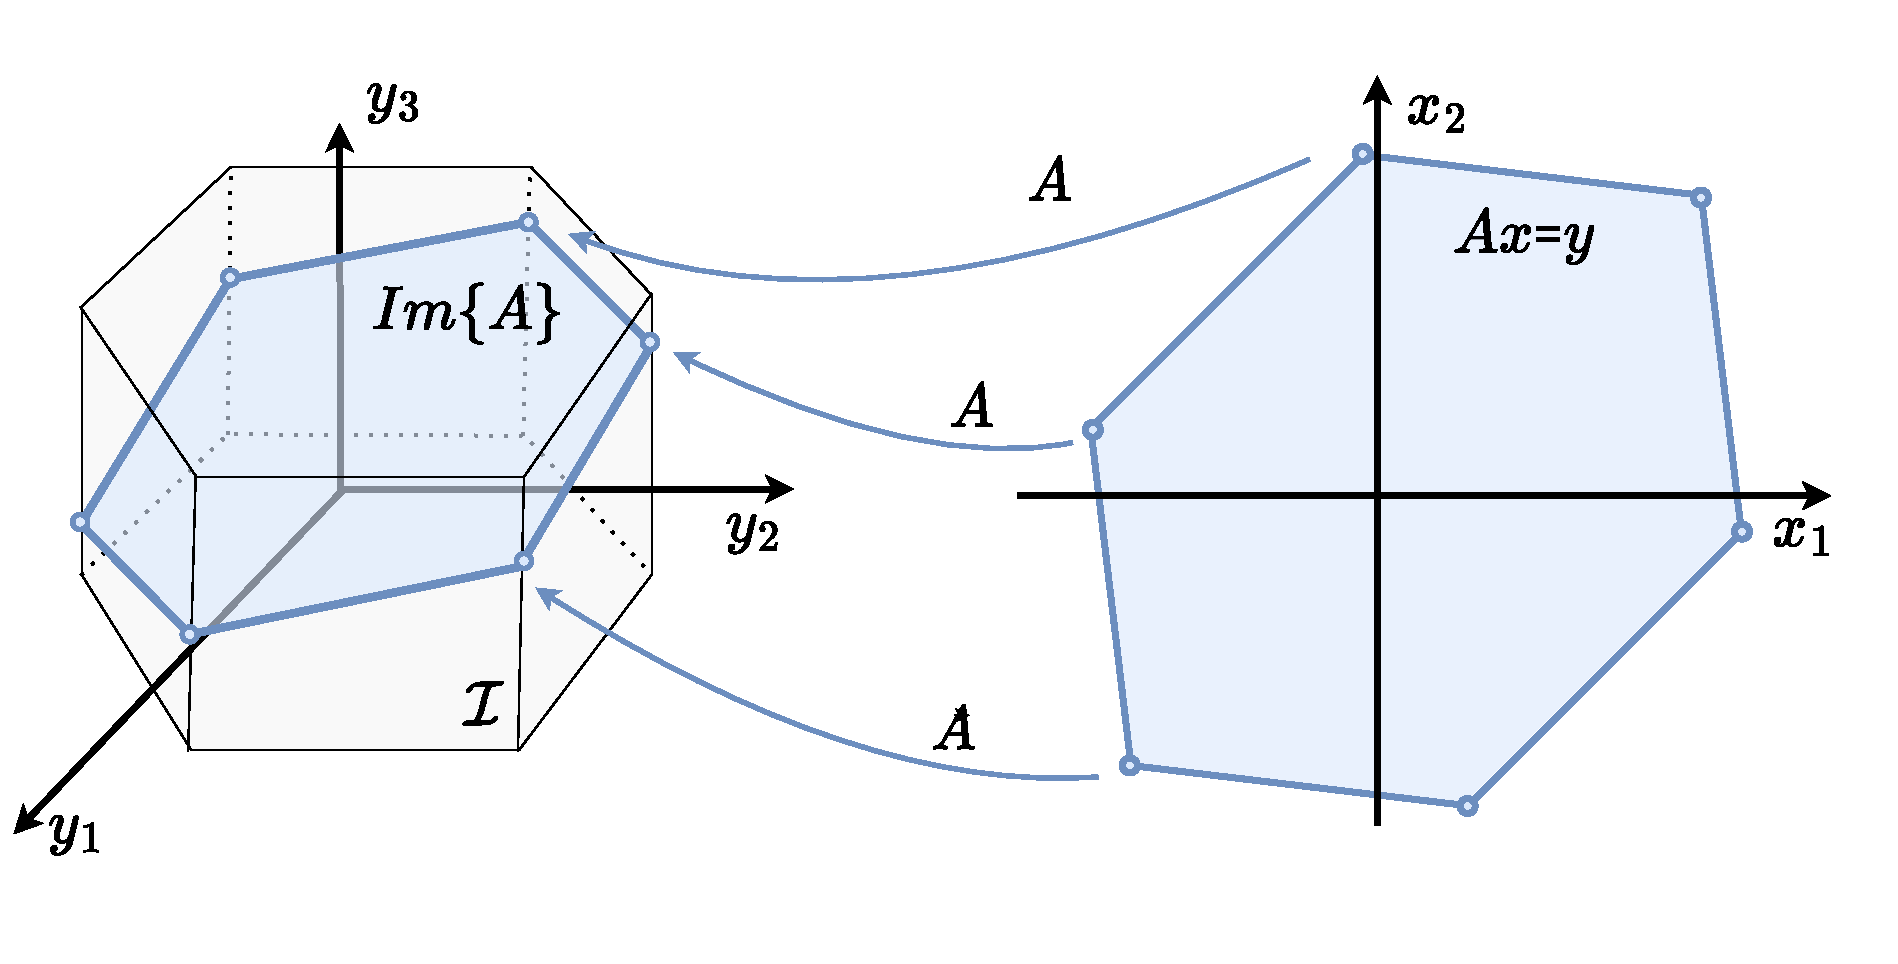
\includegraphics[width=0.7\linewidth]{Chapters/imgs/inter_poly.pdf}
    \caption{Caption}
    \label{fig:inter_poly}
\end{figure}

In the case when the input space $\mathcal{I}$ is already a polytope, given its structure, finding the $\mathcal{V}$ or $\mathcal{H}$- representation of the intersection polytope (\ref{eq:inter_poly}) varies in difficulty. The geometrical interpretation of the intersection remains very similar as in the case of the hypercube $\mathcal{I}$, however this time the image of the matrix $A$ is intersected with the polytope $\mathcal{I}$, as showon in a example on Figure \ref{fig:inter_poly}.

When the polytope $\mathcal{I}$ is defined by its $\mathcal{H}$-representation 
\begin{equation}
    \mathcal{I} = \{ \bm{y} ~|~H\bm{y} \leq \bm{d}\}
\end{equation}
then finding the $\mathcal{H}$-representation of the polytope (\ref{eq:inter_poly}) can be found by replacing the vecotor $\bm{y}$ with $A\bm{x}$
\begin{equation}
    \mathcal{P}_x=\{\bm{x} |~ HA\bm{x} \leq \bm{d} \}
    \label{eq:inter_poly_h_rep}
\end{equation}
Finding the $\mathcal{V}$-representation can then be performed using standard vertex enumeration methods such as DDM \cite{fukuda_dd}. \todo[inline]{not minimal}

In the case where the polytope $\mathcal{I}$ is defined by its $\mathcal{V}$-representation, 
\begin{equation}
    \mathcal{I} = conv\{ \bm{y}_{v1}, ~ \bm{y}_{v2},~ \ldots\}
\end{equation}
these vertices can be transformed to the $\mathcal{H}$-representation using techniques such as DDM \cite{fukuda_dd} or different convex-hull algorithms \cite{Barber1996}, which can then be used with the above described approach.

The polytope $\mathcal{I}$ in general case can have different formulation that is neither its $\mathcal{V}$ or $\mathcal{H}$-representation. For example, it might have an intersection (\ref{eq:inter_poly}) or projection (\ref{eq:proj_poly}) form, or might include additional equality and inequality constraints. In this case the same approach can be applied to $\mathcal{I}$, first transformed to the $\mathcal{H}$-representation which can then be directly used to find the $\mathcal{H}$ or $\mathcal{V}$-representation of the polytope $\mathcal{P}_x$.

In cases where the time-efficiency of finding the $\mathcal{H}$ representation of the polytope $\mathcal{I}$ or even enumerating vertices of the polytope (\ref{eq:inter_poly_h_rep}) might be not appropriate for given application, polytope approximation strategies described in Chapter \ref{ch:approximation_algos} might be a viable option.

\subsection{Projection formulation $x=By$ with polytope limits $\mathcal{I}$}

\begin{figure}[h]
    \centering
    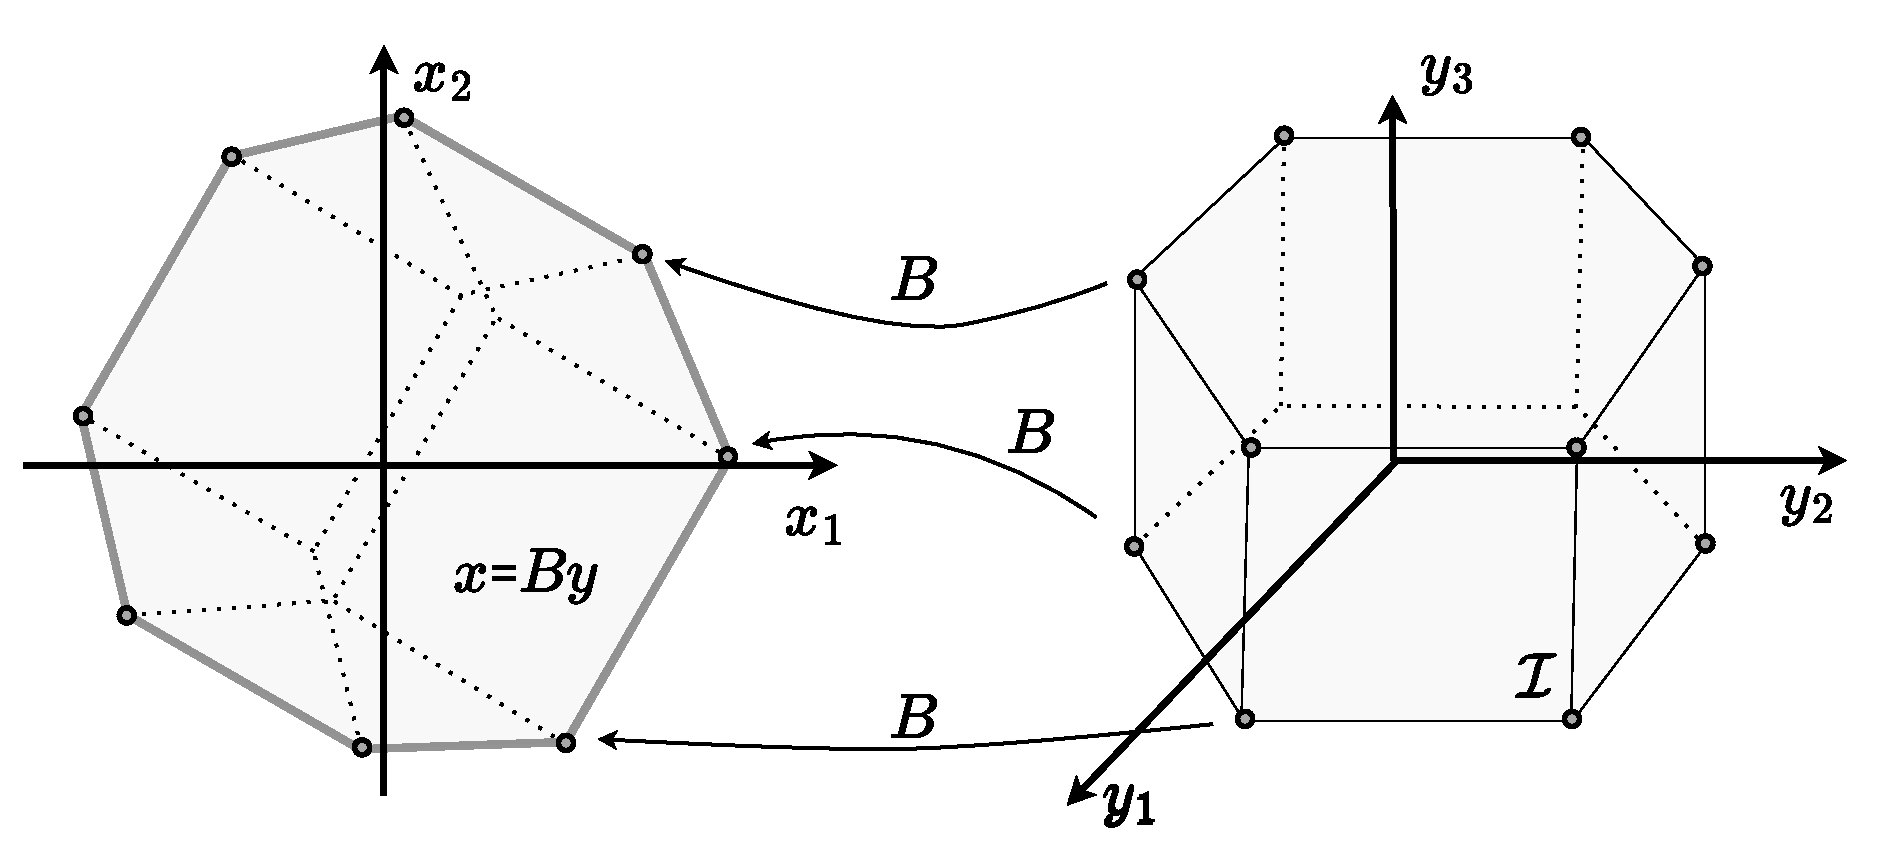
\includegraphics[width=0.7\linewidth]{Chapters/imgs/proj_poly.pdf}
    \caption{Caption}
    \label{fig:proj_poly}
\end{figure}

When the input limits $\mathcal{I}$ have a form of a polytope, depending on the way $\mathcal{I}$ is defined, there are different ways to find projection polytope (\ref{eq:proj_poly}) vertex and half-plane representation. 

If $\mathcal{I}$ is expressed with its $\mathcal{V}$-representation
\begin{equation}
    \mathcal{I} = conv\{ \bm{y}_{v1}, ~ \bm{y}_{v2},~ \ldots\}
\end{equation}
then the projection formulation polytope (\ref{eq:proj_poly}) can be found by projecting the vertices of $\mathcal{I}$ to the output space using the matrix $B$ and calculating the convex-hull of the projected vertices
\begin{equation}
    \mathcal{P}_x= conv\{ B\bm{y}_{v1}, ~ B\bm{y}_{v2},~ \ldots\}
\end{equation}
The convex-hull algorithm finds the $\mathcal{V}$-representation of the projection polytope directly, as the vertices of the polytope (\ref{eq:proj_poly}) are a subset of the projected vertices $\bm{y}_{vi}$ of the input polytope $\mathcal{I}$, as shown in the example on Figure \ref{fig:proj_poly}. 
To find the $\mathcal{H}$-representation, once the $\mathcal{V}$-representation is determined, the DDM can be used.

If the input polytope $\mathcal{I}$ is defined using its $\mathcal{H}$ representation, 
\begin{equation}
    \mathcal{I} = \{ \bm{y} ~|~H\bm{y} \leq \bm{d}\}
\end{equation}
the straight-forward approach consists in decoupling the problem and find the $\mathcal{V}$-representation first, using for example using standard vertex enumeration methods such as DDM, then follow the above described procedure to find the desired representation of the $\mathcal{P}_x$. However, if the $\mathcal{H}$-representation of the polytope $\mathcal{I}$ is available, decoupling is not necessary as the $\mathcal{H}$-representation of the polytope $\mathcal{P}_x$ can be foudn directly using the algorithms such as Fourier-Motzkin Elimination (FME) \cite{dantzig1973fourier} and Equality-Set Projection (ESP) \cite{jones2004equality}. Then if the $\mathcal{V}$-representation is required the standard vertex enumeration methods such as DDM can be used with the obtained $\mathcal{H}$-representation.

Finally, in cases where the time-efficiency of finding the $\mathcal{V}$-representation of the polytope $\mathcal{I}$ or using the DDM, FME or ESP methods might not be appropriate for given application, polytope approximation strategies described in Chapter \ref{ch:approximation_algos} might be a viable option.

\subsection{Polytope approximation strategies}
\label{ch:approximation_algos}
 
\begin{figure}[!htb]
    \centering
    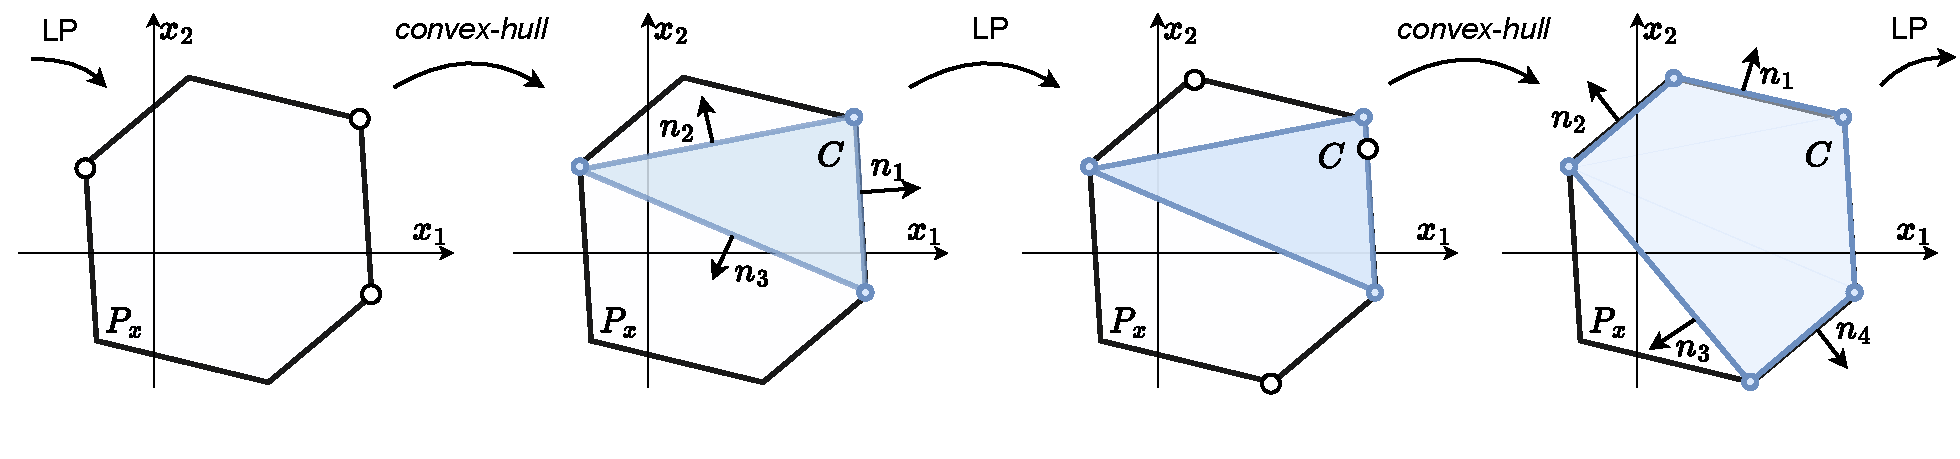
\includegraphics[width=\linewidth]{Chapters/imgs/ray_shooting.pdf}
    \caption{Caption}
    \label{fig:rsm}
\end{figure}

Exact methods, such as DDM, HPSM, FME and similar, rely on different versions of exhaustive search in the $n$-dimensional input space, having execution time exponentially related to the number of vertices and the faces of the input space bounds $\mathcal{I}$. This relationship can make them not practical for interactive in the loop applications. As the polytope based physical ability metrics $\mathcal{P}_x$ are usually defined in the low-dimensional outputs space $\bm{x}\in R^m$, several methods have been proposed performing the search in the $m$-dimensional output space. These methods are \textit{output sensitive}, having the execution time proportional to the number of vertices and the faces of the output space polytope $\mathcal{P}_x$ rather than on the input space polytope $\mathcal{I}$. 
In addition to searching in the lower dimensional output space these methods enable finding an efficient inner (or outer) approximation of the polytope $\mathcal{P}_x$ while satisfying the desired approximation accuracy. Finally, these methods evaluate the vertices and faces of the polytope $\mathcal{P}_x$ at the same time providing both $\mathcal{V}$ and $\mathcal{H}$-representation.

These methods, as introduced by Lassez et al. \cite{lassez1992quantifier, Huynh2005PracticalIO}, iteratively approximate the polytope $\mathcal{P}_x$ augmenting the approximation accuracy in each iteration. These methods, often called Ray Shooting Methods (RSM) or Convex-Hull Methods(CHM), have two phases. In the first phase an initial approximation of the polytope $\mathcal{P}_x$ is constructed finding a subset of $m+1$ vertices forming an initial $m$-dimensional convex-hull $\mathcal{C}$ approximation of the polytope $\mathcal{P}_x$. In the second phase the convex-hull approximation $\mathcal{C}$ is refined iteratively until the desired accuracy is reached. The CHM algorithms use a sequence of linear programs (LP) to find new vertices of the polytope in each iteration, followed by the convex-hull algorithm to group them to the faces. An example of the CHM algorithm in for $m=2$ output space is shown on Figure \ref{fig:rsm}.   

CHM algorithms have several limitations though. The resolution of the CHM algorithms relies on iterative application of the convex-hull algorithm which complexity grows exponentially for $m \geq 4$ \cite{Barber1996}. As a result, the applications of these methods have so far been limited to the low-dimensional output spaces $m\leq3$. Additionally, as different polytope formulations require different LP formulations, the implementations of these methods are often somewhat specific to their respective applications. 

There are several examples in the literature of using CHM based methods for improving the efficiency of different computationally expensive polytope evaluation problems. Bretl et al. \cite{Bretl2008} have proposed a CHM based algorithm for 2d ($m\!=2\!$) support region approximation for legged robot locomotion, their work has recently been extended by Audren et al. \cite{Herve2018} to the case of 3d ($m\!=3\!$) robust stability region calculation. Carmicahel et al. \cite{carmichael2011Towards, carmichael_estimating_2013} have used a simplified CHM algorithm for the calculation of the 2d ($m\!=2\!$) force capacity polytope of the human arm, based on its musculoskeltal model. Ponce and Faverjon \cite{Ponce1995} have introduced a derivative of the CHM algorithm to calculate the 2d, 2d and 4d ($m\!=2,3,4\!$) stable grasp regions for the force-closure grasp using three fingers. 

Therefore, CHM based algorithms are a promising tool for reducing complexity and improving efficiency of the polytope evaluation when the dimension $n$ of the input space is high (and/or input space limits $\mathcal{I}$ have a complex geometry) while the dimension of the output space $m$ is reasonably low $m\leq3$.

\chapter{Our contribution 1}
\chapter{Our contribution 2}

